\protect\hyperlink{main-nav}{≡} \protect\hyperlink{close-nav}{×}

\hypertarget{section-2.5-chain-rule}{%
\section{Section 2.5: Chain Rule}\label{section-2.5-chain-rule}}

There is one more type of complicated function that we will want to know
how to differentiate: composition. The Chain Rule will let us find the
derivative of a composition. (This is the last derivative rule we will
learn!)

\hypertarget{example-1}{%
\paragraph{Example 1}\label{example-1}}

Find the derivative of \textbackslash{}(
y=\textbackslash{}left(4x\^{}3+15x\textbackslash{}right)\^{}2
\textbackslash{})

This is not a simple polynomial, so we can't use the basic building
block rules yet. It is a product, so we could write it as
\textbackslash{}(y=\textbackslash{}left(4x\^{}3+15x\textbackslash{}right)\^{}2=\textbackslash{}left(4x\^{}3+15x\textbackslash{}right)\textbackslash{}left(4x\^{}3+15x\textbackslash{}right)\textbackslash{})
and use the product rule. Or we could multiply it out and simply
differentiate the resulting polynomial. I'll do it the second way:
\textbackslash{}{[} \textbackslash{}begin\{align*\} y=\&
\textbackslash{}left(4x\^{}3+15x\textbackslash{}right)\^{}2\textbackslash{}\textbackslash{}
=\& 16x\^{}6+120x\^{}4+225x\^{}2\textbackslash{}\textbackslash{} y'=\&
96x\^{}5+480x\^{}3+450x \textbackslash{}end\{align*\}
\textbackslash{}{]}

Now suppose we want to find the derivative of
\textbackslash{}(y=\textbackslash{}left(4x\^{}3+15x\textbackslash{}right)\^{}\{20\}\textbackslash{}).
We \textbf{could} write it as a product with 20 factors and use the
product rule, or we \textbf{could} multiply it out. But I don't want to
do that, do you?

We need an easier way, a rule that will handle a composition like this.
The Chain Rule is a little complicated, but it saves us the much more
complicated algebra of multiplying something like this out. It will also
handle compositions where it wouldn't be possible to ``multiply it
out.''

The Chain Rule is a common place for students to make mistakes. Part of
the reason is that the notation takes a little getting used to. And part
of the reason is that students often forget to use it when they should.
When should you use the Chain Rule? Almost every time you take a
derivative.

To view this video please enable JavaScript, and consider upgrading to a
web browser that \href{http://videojs.com/html5-video-support/}{supports
HTML5 video}

\hypertarget{derivative-rules-chain-rule}{%
\paragraph{Derivative Rules: Chain
Rule}\label{derivative-rules-chain-rule}}

In what follows, \textbackslash{}(f\textbackslash{}) and
\textbackslash{}(g\textbackslash{}) are differentiable functions with
\textbackslash{}( y=f(u) \textbackslash{}) and \textbackslash{}( u=g(x)
\textbackslash{}).

\hypertarget{chain-rule-leibniz-notation}{%
\subparagraph{Chain Rule (Leibniz
notation)}\label{chain-rule-leibniz-notation}}

\textbackslash{}{[}\textbackslash{}frac\{dy\}\{dx\}=\textbackslash{}frac\{dy\}\{du\}\textbackslash{}cdot\textbackslash{}frac\{du\}\{dx\}\textbackslash{}{]}

Notice that the \textbackslash{}(du\textbackslash{})'s seem to cancel.
This is one advantage of the Leibniz notation -- it can remind you of
how the chain rule chains together.

\hypertarget{chain-rule-using-prime-notation}{%
\subparagraph{Chain Rule (using prime
notation)}\label{chain-rule-using-prime-notation}}

\textbackslash{}{[}f'(x)=f'(u)\textbackslash{}cdot
g'(x)=f'\textbackslash{}left(g(x)\textbackslash{}right)\textbackslash{}cdot
g'(x)\textbackslash{}{]}

\hypertarget{chain-rule-in-words}{%
\subparagraph{Chain Rule (in words)}\label{chain-rule-in-words}}

The derivative of a composition is the derivative of the outside (with
the inside staying the same) TIMES the derivative of the inside.

I recite the version in words each time I take a derivative, especially
if the function is complicated.

\hypertarget{example-2}{%
\paragraph{Example 2}\label{example-2}}

Find the derivative of \textbackslash{}(
y=\textbackslash{}left(4x\^{}3+15x\textbackslash{}right)\^{}2
\textbackslash{})

This is the same one we did before by multiplying out. This time, let's
use the Chain Rule: The inside function is what appears inside the
parentheses: \textbackslash{}( 4x\^{}3+15x \textbackslash{}). The
outside function is the first thing we find as we come in from the
outside -- it's the square function,
\textbackslash{}((\textbackslash{}text\{inside\})\^{}2\textbackslash{}).

The derivative of this outside function is
\textbackslash{}((2\textbackslash{}cdot\textbackslash{}text\{inside\})\textbackslash{}).
Now using the chain rule, the derivative of our original function is
\textbackslash{}((2\textbackslash{}cdot\textbackslash{}text\{inside\})\textbackslash{})
TIMES the derivative of the inside (which is \textbackslash{}(
12x\^{}2+15 \textbackslash{})): \textbackslash{}{[}
y'=2\textbackslash{}left(4x\^{}3+15x\textbackslash{}right)\textbackslash{}left(12x\^{}2+15
\textbackslash{}right)\textbackslash{}{]}

If you multiply this out, you get the same answer we got before. Hurray!
Algebra works!

\hypertarget{example-3}{%
\paragraph{Example 3}\label{example-3}}

Find the derivative of \textbackslash{}(
y=\textbackslash{}left(4x\^{}3+15x\textbackslash{}right)\^{}\{20\}
\textbackslash{}).

Now we have a way to handle this one. It's the derivative of the outside
TIMES the derivative of the inside.

The outside function is \textbackslash{}(
\textbackslash{}left(\textbackslash{}text\{inside\}\textbackslash{}right)\^{}\{20\}
\textbackslash{}), which has derivative \textbackslash{}(
20\textbackslash{}left(\textbackslash{}text\{inside\}\textbackslash{}right)\^{}\{19\}\textbackslash{}),
so
\textbackslash{}{[}y'=20\textbackslash{}left(4x\^{}3+15x\textbackslash{}right)\^{}\{19\}\textbackslash{}left(12x\^{}2+15\textbackslash{}right).\textbackslash{}{]}

\hypertarget{example-4}{%
\paragraph{Example 4}\label{example-4}}

Differentiate \textbackslash{}( y=e\^{}\{x\^{}2+5\} \textbackslash{}).

This isn't a simple exponential function; it's a composition. Typical
calculator or computer syntax can help you see what the ``inside''
function is here. On a TI calculator, for example, when you push the
\textbackslash{}( e\^{}x \textbackslash{}) key, it opens up parentheses:
e\^{}( . This tells you that the "inside" of the exponential function is
the exponent. Here, the inside is the exponent \textbackslash{}(
x\^{}2+5 \textbackslash{}). Now we can use the Chain Rule: We want the
derivative of the outside TIMES the derivative of the inside. The
outside is the ``\textbackslash{}(e\textbackslash{}) to the something''
function, so its derivative is the same thing. The derivative of what's
inside is \textbackslash{}(2x\textbackslash{}). So
\textbackslash{}{[}\textbackslash{}frac\{d\}\{dx\}\textbackslash{}left(
e\^{}\{x\^{}2+5\} \textbackslash{}right)= \textbackslash{}left(
e\^{}\{x\^{}2+5\} \textbackslash{}right)\textbackslash{}cdot
(2x).\textbackslash{}{]}

\hypertarget{example-5}{%
\paragraph{Example 5}\label{example-5}}

The table gives values for \textbackslash{}(f\textbackslash{}) ,
\textbackslash{}(f'\textbackslash{}) ,
\textbackslash{}(g\textbackslash{}), and
\textbackslash{}(g'\textbackslash{}) at a number of points. Use these
values to determine \textbackslash{}(( f \textbackslash{}circ g
)(x)\textbackslash{}) and \textbackslash{}(( f \textbackslash{}circ g )
'(x)\textbackslash{}) at \textbackslash{}(x = -1\textbackslash{}) and 0.

\begin{longtable}[]{@{}lllllll@{}}
\toprule
\endhead
\textbackslash{}( x \textbackslash{}) & \textbackslash{}( f(x)
\textbackslash{}) & \textbackslash{}( g(x) \textbackslash{}) &
\textbackslash{}( f'(x) \textbackslash{}) & \textbackslash{}( g'(x)
\textbackslash{}) & \textbackslash{}((f\textbackslash{}circ
g)(x)\textbackslash{}) & \textbackslash{}((g\textbackslash{}circ
f)(x)\textbackslash{})\tabularnewline
-1 & 2 & 3 & 1 & 0 & &\tabularnewline
0 & -1 & 1 & 3 & 2 & &\tabularnewline
1 & 1 & 0 & -1 & 3 & &\tabularnewline
2 & 3 & -1 & 0 & 1 & &\tabularnewline
3 & 0 & 2 & 2 & -1 & &\tabularnewline
\bottomrule
\end{longtable}

\textbackslash{}{[} \textbackslash{}begin\{align*\}
(f\textbackslash{}circ g)(-1)=\&
f\textbackslash{}left(g(-1)\textbackslash{}right)=f(3)=0\textbackslash{}\textbackslash{}
(f\textbackslash{}circ g)(0)=\&
f\textbackslash{}left(g(0)\textbackslash{}right)=f(1)=1\textbackslash{}\textbackslash{}
(f\textbackslash{}circ g)'(-1)=\&
f'\textbackslash{}left(g(-1)\textbackslash{}right)\textbackslash{}cdot
g'(-1)=f'(3)\textbackslash{}cdot (0)=(2)(0)=0 \textbackslash{}text\{
and\}\textbackslash{}\textbackslash{} (f\textbackslash{}circ g)'(0)=\&
f'\textbackslash{}left(g(0)\textbackslash{}right)\textbackslash{}cdot
g'(0)=f'(1)\textbackslash{}cdot (2)=(-1)(2)=-2
\textbackslash{}end\{align*\} \textbackslash{}{]}

To view this video please enable JavaScript, and consider upgrading to a
web browser that \href{http://videojs.com/html5-video-support/}{supports
HTML5 video}

\hypertarget{example-6}{%
\paragraph{Example 6}\label{example-6}}

If 2400 people now have a disease, and the number of people with the
disease appears to double every 3 years, then the number of people
expected to have the disease in \textbackslash{}(t\textbackslash{})
years is \textbackslash{}( y=2400\textbackslash{}cdot 2\^{}\{t/3\}
\textbackslash{}).

\begin{enumerate}
\tightlist
\item
  How many people are expected to have the disease in 2 years?
\item
  When are 50,000 people expected to have the disease?
\item
  How fast is the number of people with the disease expected to grow now
  and 2 years from now?
\end{enumerate}

\begin{enumerate}
\tightlist
\item
  In 2 years, \textbackslash{}(y = 2400\textbackslash{}cdot 2\^{}\{2/3\}
  \textbackslash{}approx 3,810\textbackslash{}) people.
\item
  We know \textbackslash{}(y = 50,000\textbackslash{}), and we need to
  solve \textbackslash{}(50,000 = 2400\textbackslash{}cdot
  2\^{}\{t/3\}\textbackslash{}) for \textbackslash{}(t\textbackslash{}).
  We could start by isolating the exponential by dividing both sides by
  2400, \textbackslash{}{[} \textbackslash{}begin\{align*\}
  \textbackslash{}frac\{50000\}\{2400\}=\& 2\^{}\{t/3\}
  \textbackslash{}\textbackslash{}
  \textbackslash{}ln\textbackslash{}left(\textbackslash{}frac\{50000\}\{2400\}\textbackslash{}right)=\&
  \textbackslash{}ln\textbackslash{}left(2\^{}\{t/3\}\textbackslash{}right)
  \textbackslash{}qquad \textbackslash{}text\{(Taking the natural log of
  both sides.)\}\textbackslash{}\textbackslash{}
  \textbackslash{}ln\textbackslash{}left(\textbackslash{}frac\{50000\}\{2400\}\textbackslash{}right)=\&
  \textbackslash{}frac\{t\}\{3\}\textbackslash{}ln(2)
  \textbackslash{}qquad \textbackslash{}text\{(Using the exponent
  property for logs.)\}\textbackslash{}\textbackslash{} t=\&
  \textbackslash{}frac\{3\textbackslash{}ln\textbackslash{}left(\textbackslash{}frac\{50000\}\{2400\}\textbackslash{}right)\}\{\textbackslash{}ln(2)\}\textbackslash{}approx
  13.14\textbackslash{}text\{ years\}\textbackslash{}qquad
  \textbackslash{}text\{(Solving for \textbackslash{}( t
  \textbackslash{}).)\} \textbackslash{}end\{align*\}
  \textbackslash{}{]} We expect 50,000 people to have the disease about
  13.14 years from now.
\item
  This is asking for
  \textbackslash{}(\textbackslash{}frac\{dy\}\{dt\}\textbackslash{})
  when \textbackslash{}(t =\textbackslash{}) 0 and 2 years. Using the
  chain rule, \textbackslash{}{[} \textbackslash{}begin\{align*\}
  \textbackslash{}frac\{dy\}\{dt\}=\&
  \textbackslash{}frac\{d\}\{dt\}\textbackslash{}left(2400\textbackslash{}cdot
  2\^{}\{t/3\}\textbackslash{}right) \textbackslash{}\textbackslash{}
  =\& 2400\textbackslash{}cdot 2\^{}\{t/3\}\textbackslash{}cdot
  \textbackslash{}ln(2)\textbackslash{}cdot\textbackslash{}frac\{1\}\{3\}
  \textbackslash{}\textbackslash{} \textbackslash{}approx\&
  554.5\textbackslash{}cdot 2\^{}\{t/3\} \textbackslash{}end\{align*\}
  \textbackslash{}{]} So, at \textbackslash{}( t=0 \textbackslash{}) the
  rate of growth of the disease is approximately
  \textbackslash{}(554.5\textbackslash{}cdot 2\^{}0
  \textbackslash{}approx 554.5\textbackslash{}) people/year. In 2 years
  the rate of growth will be approximately
  \textbackslash{}(554.5\textbackslash{}cdot 2\^{}\{2/3\}
  \textbackslash{}approx 880\textbackslash{}) people/year.
\end{enumerate}

\hypertarget{derivatives-of-complicated-functions}{%
\subsection{Derivatives of Complicated
Functions}\label{derivatives-of-complicated-functions}}

You're now ready to take the derivative of some mighty complicated
functions. But how do you tell what rule applies first? Work your way in
from the outside -- what do you encounter first? That's the first rule
you need. Use the Product, Quotient, and Chain Rules to peel off the
layers, one at a time, until you're all the way inside.

\hypertarget{example-7}{%
\paragraph{Example 7}\label{example-7}}

Find \textbackslash{}(
\textbackslash{}frac\{d\}\{dx\}\textbackslash{}left(
e\^{}\{3x\}\textbackslash{}cdot\textbackslash{}ln(5x+7)
\textbackslash{}right) \textbackslash{})

Coming in from the outside, we see that this is a product of two
(complicated) functions. So we'll need the Product Rule first. we'll
fill in the pieces we know, and then we can figure the rest as separate
steps and substitute in at the end:
\textbackslash{}{[}\textbackslash{}frac\{d\}\{dx\}\textbackslash{}left(
e\^{}\{3x\}\textbackslash{}cdot\textbackslash{}ln(5x+7)
\textbackslash{}right)=\textbackslash{}left(
\textbackslash{}frac\{d\}\{dx\}\textbackslash{}left(
e\^{}\{3x\}\textbackslash{}right)\textbackslash{}right)\textbackslash{}cdot\textbackslash{}ln(5x+7)+
e\^{}\{3x\}\textbackslash{}cdot
\textbackslash{}left(\textbackslash{}frac\{d\}\{dx\}\textbackslash{}left(\textbackslash{}ln(5x+7)
\textbackslash{}right)\textbackslash{}right)\textbackslash{}{]}

Now as separate steps, we'll find
\textbackslash{}{[}\textbackslash{}frac\{d\}\{dx\}\textbackslash{}left(
e\^{}\{3x\}\textbackslash{}right)=3e\^{}\{3x\} \textbackslash{}quad
\textbackslash{}text\{ (using the Chain Rule)\}\textbackslash{}{]} and
\textbackslash{}{[}\textbackslash{}frac\{d\}\{dx\}\textbackslash{}left(\textbackslash{}ln(5x+7)
\textbackslash{}right)=\textbackslash{}frac\{1\}\{5x+7\}\textbackslash{}cdot
5 \textbackslash{}quad \textbackslash{}text\{ (also using the Chain
Rule)\}.\textbackslash{}{]}

Finally, to substitute these in their
places:\textbackslash{}{[}\textbackslash{}frac\{d\}\{dx\}\textbackslash{}left(
e\^{}\{3x\}\textbackslash{}cdot\textbackslash{}ln(5x+7)
\textbackslash{}right)=\textbackslash{}left(
3e\^{}\{3x\}\textbackslash{}right)\textbackslash{}cdot\textbackslash{}ln(5x+7)+
e\^{}\{3x\}\textbackslash{}cdot
\textbackslash{}left(\textbackslash{}frac\{1\}\{5x+7\}\textbackslash{}cdot
5\textbackslash{}right)\textbackslash{}{]}

(We can stop here -- we don't need to try to simplify any further.)

\hypertarget{example-8}{%
\paragraph{Example 8}\label{example-8}}

Differentiate \textbackslash{}(
z=\textbackslash{}left(\textbackslash{}dfrac\{3t\^{}3\}\{e\^{}t(t-1)\}\textbackslash{}right)\^{}4
\textbackslash{})

Don't panic! As we come in from the outside, what's the first thing we
encounter? It's that fourth power. That tells us that this is a
composition, a (complicated) function raised to the fourth power.

Step One: Use the Chain Rule. The derivative of the outside TIMES the
derivative of the inside:
\textbackslash{}{[}\textbackslash{}frac\{dz\}\{dt\}=\textbackslash{}frac\{d\}\{dt\}\textbackslash{}left(\textbackslash{}frac\{3t\^{}3\}\{e\^{}t(t-1)\}\textbackslash{}right)\^{}4=4\textbackslash{}left(\textbackslash{}frac\{3t\^{}3\}\{e\^{}t(t-1)\}\textbackslash{}right)\^{}3\textbackslash{}cdot
\textbackslash{}frac\{d\}\{dt\}\textbackslash{}left(\textbackslash{}frac\{3t\^{}3\}\{e\^{}t(t-1)\}\textbackslash{}right)\textbackslash{}{]}

Now we're one step inside, and we can concentrate on just the
\textbackslash{}(
\textbackslash{}frac\{d\}\{dt\}\textbackslash{}left(\textbackslash{}frac\{3t\^{}3\}\{e\^{}t(t-1)\}\textbackslash{}right)
\textbackslash{}) part. Now, as you come in from the outside, the first
thing you encounter is a quotient -- this is the quotient of two
(complicated) functions.

Step Two: Use the Quotient Rule. The derivative of the numerator is
straightforward, so we can just calculate it. The derivative of the
denominator is a bit trickier, so we'll leave it for now:
\textbackslash{}{[}
\textbackslash{}frac\{d\}\{dt\}\textbackslash{}left(\textbackslash{}frac\{3t\^{}3\}\{e\^{}t(t-1)\}\textbackslash{}right)=\textbackslash{}frac\{\textbackslash{}left(
9t\^{}2 \textbackslash{}right)\textbackslash{}left( e\^{}t(t-1)
\textbackslash{}right)-\textbackslash{}left( 3t\^{}3
\textbackslash{}right)\textbackslash{}left(
\textbackslash{}frac\{d\}\{dt\}\textbackslash{}left( e\^{}t(t-1)
\textbackslash{}right)
\textbackslash{}right)\}\{\textbackslash{}left(e\^{}t(t-1)\textbackslash{}right)\^{}2\}
\textbackslash{}{]}

Now we've gone one more step inside, and we can concentrate on just the
\textbackslash{}( \textbackslash{}frac\{d\}\{dt\}\textbackslash{}left(
e\^{}t(t-1) \textbackslash{}right) \textbackslash{}) part, which
involves a product.

Step Three: Use the Product Rule: \textbackslash{}{[}
\textbackslash{}frac\{d\}\{dt\}\textbackslash{}left(
e\^{}t(t-1)\textbackslash{}right) = \textbackslash{}left( e\^{}t
\textbackslash{}right)(t-1)+\textbackslash{}left( e\^{}t
\textbackslash{}right)(1)\textbackslash{}{]}

And now we're all the way in -- no more derivatives to take!

Step Four: Now it's just a question of substituting back -- be careful
now!

\textbackslash{}{[} \textbackslash{}frac\{d\}\{dt\}\textbackslash{}left(
e\^{}t(t-1)\textbackslash{}right) = \textbackslash{}left( e\^{}t
\textbackslash{}right)(t-1)+\textbackslash{}left( e\^{}t
\textbackslash{}right)(1) \textbackslash{}{]} so \textbackslash{}{[}
\textbackslash{}frac\{d\}\{dt\}\textbackslash{}left(\textbackslash{}frac\{3t\^{}3\}\{e\^{}t(t-1)\}\textbackslash{}right)=\textbackslash{}frac\{\textbackslash{}left(
9t\^{}2 \textbackslash{}right)\textbackslash{}left( e\^{}t(t-1)
\textbackslash{}right)-\textbackslash{}left( 3t\^{}3
\textbackslash{}right)\textbackslash{}left( \textbackslash{}left( e\^{}t
\textbackslash{}right)(t-1)+\textbackslash{}left( e\^{}t
\textbackslash{}right)(1)
\textbackslash{}right)\}\{\textbackslash{}left(e\^{}t(t-1)\textbackslash{}right)\^{}2\}
\textbackslash{}{]} so
\textbackslash{}{[}\textbackslash{}frac\{dz\}\{dt\}=\textbackslash{}frac\{d\}\{dt\}\textbackslash{}left(\textbackslash{}frac\{3t\^{}3\}\{e\^{}t(t-1)\}\textbackslash{}right)\^{}4=4\textbackslash{}left(\textbackslash{}frac\{3t\^{}3\}\{e\^{}t(t-1)\}\textbackslash{}right)\^{}3\textbackslash{}cdot
\textbackslash{}left( \textbackslash{}frac\{\textbackslash{}left(
9t\^{}2 \textbackslash{}right)\textbackslash{}left( e\^{}t(t-1)
\textbackslash{}right)-\textbackslash{}left( 3t\^{}3
\textbackslash{}right)\textbackslash{}left( \textbackslash{}left( e\^{}t
\textbackslash{}right)(t-1)+\textbackslash{}left( e\^{}t
\textbackslash{}right)(1)
\textbackslash{}right)\}\{\textbackslash{}left(e\^{}t(t-1)\textbackslash{}right)\^{}2\}
\textbackslash{}right)\textbackslash{}{]}

Phew!

\hypertarget{what-if-the-derivative-doesnt-exist}{%
\subsection{What if the Derivative Doesn't
Exist?}\label{what-if-the-derivative-doesnt-exist}}

\hypertarget{differentiable}{%
\paragraph{Differentiable}\label{differentiable}}

A function is called \textbf{differentiable} at a point if its
derivative exists at that point.

We've been acting as if derivatives exist everywhere for every function.
This is true for most of the functions that you will run into in this
class. But there are some common places where the derivative doesn't
exist.

Remember that the derivative is the slope of the tangent line to the
curve. That's what to think about.

Where can a slope not exist? \textbf{If the tangent line is vertical,
the derivative will not exist.}

\hypertarget{example-9}{%
\paragraph{Example 9}\label{example-9}}

Show that \textbackslash{}(
f(x)=\textbackslash{}sqrt{[}3{]}\{x\}=x\^{}\{1/3\} \textbackslash{}) is
not differentiable at \textbackslash{}(x = 0\textbackslash{}).

Finding the derivative, \textbackslash{}(
f(x)=\textbackslash{}frac\{1\}\{3\}x\^{}\{-2/3\}=\textbackslash{}frac\{1\}\{3x\^{}\{2/3\}\}
\textbackslash{}). At \textbackslash{}(x = 0\textbackslash{}), this
function is undefined. From the graph, we can see that the tangent line
to this curve at \textbackslash{}(x = 0\textbackslash{}) is vertical
with undefined slope, which is why the derivative does not exist at
\textbackslash{}(x = 0\textbackslash{}).

\begin{figure}
\centering
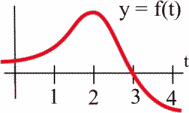
\includegraphics{images/image037.png}
\caption{}
\end{figure}

Where can a tangent line not exist?

\textbf{If there is a sharp corner (cusp) in the graph, the derivative
will not exist at that point} because there is no well-defined tangent
line (a teetering tangent, if you will).

\textbf{If there is a discontinuity in the graph} (a jump, a break, a
hole in the graph, or a vertical asymptote), the tangent line will be
different on either side and \textbf{the derivative will not exist at
that point}.

\hypertarget{example-10}{%
\paragraph{Example 10}\label{example-10}}

Show that \textbackslash{}( f(x)=\textbar{}x\textbar{} \textbackslash{})
is not differentiable at \textbackslash{}(x = 0\textbackslash{}).

On the left side of the graph, the slope of the line is -1. On the right
side of the graph, the slope is +1. There is no well-defined tangent
line at the sharp corner at \textbackslash{}(x = 0\textbackslash{}), so
the function is not differentiable at that point.

\begin{figure}
\centering
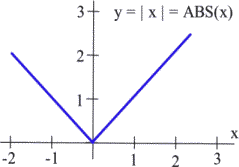
\includegraphics{images/image038.png}
\caption{}
\end{figure}

To view this video please enable JavaScript, and consider upgrading to a
web browser that \href{http://videojs.com/html5-video-support/}{supports
HTML5 video}

\begin{longtable}[]{@{}ll@{}}
\toprule
\endhead
\href{section2-4.php}{← Previous Section} & \href{section2-6.php}{Next
Section →}\tabularnewline
\bottomrule
\end{longtable}
